\chapter{Estado de la Cuestión}
\label{cap:estadoDeLaCuestion}
En este capítulo se presenta el estado del arte de los distintos elementos que componen el trabajo. Estos campos son los comportamientos de \glspl{npc} en videojuegos, los modelos de lenguaje y la generación automática de comportamientos.

\section{Comportamientos de \glspl{npc} en videojuegos}
Como bien se ha mencionado en la sección \ref{cap:introduccion}, a medida que los videojuegos han ido creciendo y evolucionando se han tenido que utilizar diferentes técnicas para modelar comportamientos cada vez más grandes y complejos, como se puede ver en \cite{AIGames}.
\subsection{Máquinas de estado finitas}
Las máquinas de estados finitas (FSM según las siglas en inglés de Finite State Machine) se definen según \cite{FSMDef} como un conjunto de estados $s_i$ y un conjunto de transiciones $s_i, s_j$ que están definidas por una relación de tipo acción/condición, donde la condición actúa como el evento desencadenante para realizar la transición y la acción representa la tarea específica que se ejecuta al cambiar de estado.
Según su definición se puede ver que resulta muy útil para modelar el comportamiento en los videojuegos, como se puede ver en la figura \ref{fig:FSMNPC}, ya que se pueden ver a los \glspl{npc} como agentes que realizan acciones (permanecen en estados) constantemente, siendo las transiciones la terminación de las acciones (cuando pasan a un estado siguiente) o un factor externo.

\begin{figure}[H]
    \centering
    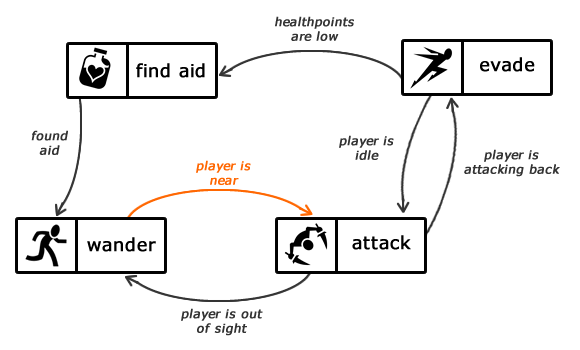
\includegraphics[width=0.75\textwidth]{Imagenes/Bitmap/FSMNPC.png}
    \caption[Ejemplo de un FSM para videojuegos]{Ejemplo de un comportamiento típico de un \glspl{npc} mediante una FSM. Fuente: \url{https://code.tutsplus.com/es/maquinas-de-estados-finitos-teoria-e-implementacion--gamedev-11867t} }
    \label{fig:FSMNPC}
\end{figure}

Esto se puede ver en trabajos como \cite{FSM-NPC1}, donde los autores presentan un videojuego en el que implementan las FSM en diferentes \glspl{npc} para que muestren un comportamiento más consistente, realista y reactivo por su simplicidad a la hora de desarrollar, dando como resultado un comportamiento inteligente y autónomo.
Otro ejemplo del uso histórico de las FSMs en videojuegos se puede ver en \cite{FSM-NPC2}, donde los autores implementan una FSM con probabilidad de transiciones distinta a 1 para emular de forma más realista el comportamiento de caza de los lobos, logrando así una experiencia más realista en inmersiva para el usuario.
Sin embargo, las FSM no están tan extendidas actualmente, ya que autores como \cite{FSM-MAL} están de acuerdo en que las FSM tienen un problema de reutilización, flexibilidad y escalabilidad con comportamientos complejos.
Aún así, actualmente se siguen utilizando como se puede ver en trabajos recientes como \cite{FSM-NPC3}, donde implementan FSM de forma clásica para \glspl{npc} o en \cite{FSM-ML}, donde combinan FSM con técnicas de Machine Learning como Q-Learning y DQN para controlar \glspl{npc} de un \gls{rpg}.

\subsection{Máquinas de estado finitas jerárquicas}
Las máquinas de estado finitas jerárquicas (HFSM por las siglas en inglés de Hierarchical Finite State Machines) se define en \cite{HFSM} como una extensión de una FSM cuyos estados puedan ser otras FSM contenidas (llamados ``superestados'').
Aunque todas las HFSM se pueden convertir en FSM mediante un proceso de \textit{flattering} reemplazando de forma recursiva los superestados por sus máquinas internas, las HFSM han solucionado probleamas de reutilización de componentes y simplicidad descriptiva.
Esta reutilización ha permitido que se extendiese su uso en videojuegos, como mencionan los autores en el trabajo citado anteriormente \cite{FSM-MAL}, con un rendimiento ligeramente mejor o similar a las FSM, como pudieron comprobar los autores en una comparativa realizada en \cite{FSMvsHFSM}.
En la figura \ref{fig:HFSMGame} se muestra un ejemplo de una HFSM en videojuegos.

\begin{figure}[H]
    \centering
    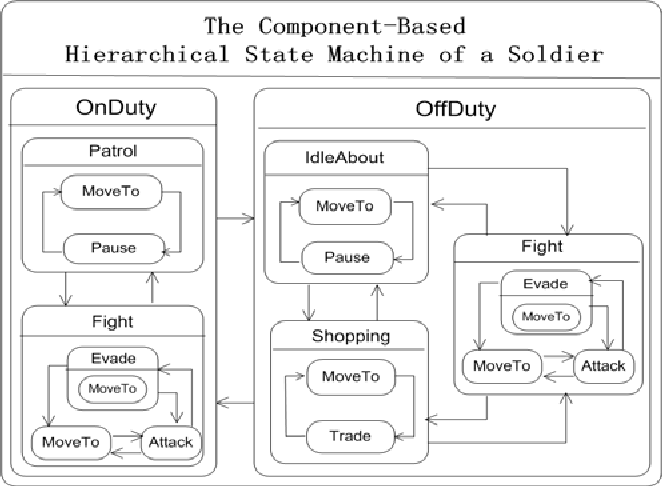
\includegraphics[width=0.75\textwidth]{Imagenes/Bitmap/HFSMGame.png}
    \caption[Ejemplo de una HFSM en videojuegos]{Ejemplo de un comportamiento de un \gls{npc} modelado en una HFSM. Fuente: \cite{FSM-MAL}.}
    \label{fig:HFSMGame}
\end{figure}

De forma comercial también se han usado las HFSM, como se puede ver en \cite{Doom}.
Otra forma de uso de las HFSM en vidoejuegos no es para comportamientos de \glspl{npc}, sino para simplificar el sistema de animaciones de videojuegos, como se puede ver en trabajos como \cite{HFSMAnim}.
El motor de videojuegos Unity Engine también estructura su sistema de animaciones\footnotemark en forma de HFSM para la simplicidad del usuario, como se puede apreciar en el estado de color naranja (estado ``Idle'') de la figura \ref{fig:HFSMUnity}.

\begin{figure}[H]
    \centering
    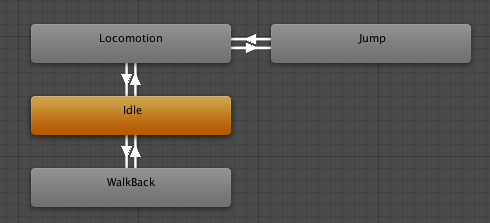
\includegraphics[width=0.75\textwidth]{Imagenes/Bitmap/StateMachineUnity.png}
    \caption[Captura del sistema de animaciones de Unity Engine]{Captura del sistema de animaciones de Unity, estructurado en forma de una HFSM en la que los nodos naranja son ``superestados''. Fuente: \url{https://docs.unity3d.com/560/Documentation/Manual/StateMachineBasics.html} }
    \label{fig:HFSMUnity}
\end{figure}

\footnotetext{Enlace a la documentación de Unity: \url{https://docs.unity3d.com/6000.7/Documentation/Manual/AnimationStateMachines.html}}

A pesar de aliviar parcialmente el problema de la duplicidad de código, autores como \cite{BTGames} argumentan que las HFSM siguen manteniendo problemas de escalabilidad y reutilización en videojuegos; y en el trabajo de \cite{HFSMvsBT} los autores comentan que sigue siendo dificil de escalar.

\subsection{Árboles de comportamiento}
Los árboles de comportamiento (conocidos como \glspl{BT}) se definen en \cite{BTDef} como árboles dirigidos formados por dos tipos de nodos: nodos hoja y nodos de composición en las que las transiciones no son unidireccionales (a diferencia de las FSM y las HFSM), sino llamadas de función bidireccionales en las que el nodo padre envía una señal periódica de activación y el hijo le responde con tres posibles estados: ``Success'', ``Failure'' o ``Running''.
Un ejemplo de \gls{BT} lo podemos encontrar en la figura \ref{EjBT}.

\begin{figure}[H]
    \centering
    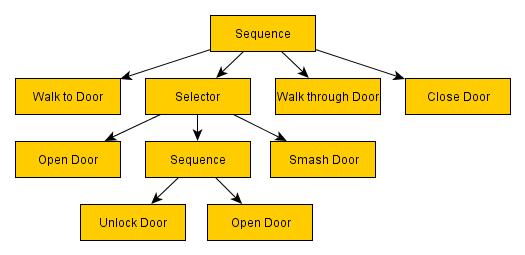
\includegraphics[width=0.75\textwidth]{Imagenes/Bitmap/BT.png}
    \caption[Ejemplo de \gls{BT}]{Ejemplo de un \gls{BT} para un \gls{npc} que debe pasar por una puerta. Fuente: \url{https://outforafight.wordpress.com/2014/07/15/behaviour-behavior-trees-for-ai-dudes-part-1/} }
    \label{fig:EjBT}
\end{figure}

Como podemos ver en \cite{BTOg}, los \glspl{BT} surgieron en el mundo de la programación de \gls{ia} de los vidoejuegos (estableciendo el videojuego Halo 2 como hito histórico) como forma de solucionar los problemas de escalabilidad, acoplamiento, adaptabilidad y reutilización que presentaban las FSM.
Además, el mismo artículo comenta que este modelo resultó ser muy valioso también para la robótica, como menciona también la revisión de \cite{BTRev} o en trabajos como \cite{BTRob}.
Actualmente hay bastante literatura sobre \glspl{BT}, sus implementaciones y posibles mejoras.
Por ejemplo, el trabajo de \cite{EDBT} nos habla de \glspl{BT} que no son evaluados cada tick sino cuando sucede un evento (llamados Event-Driven Behavior Trees o EDBT), mejorando así la cooperación en entornos multi-agente.
También podemos ver en el trabajo de \cite{BTVarios} varias ampliaciones a los \glspl{BT} en videojuegos, como los EDBT, los árboles de comportamiento emocionales (EmBT) que altera dinámicamente la prioridad de los nodos hijos dependiendo de pesos emocionales (aportando así más humanidad a los \glspl{npc}) y la evolución de los comportamientos (Evolving Behavior), \glspl{BT} que utilizan la programación genética para automatizar su optimización.

Aunque artículos como \cite{BTEstandar} hablan del uso de los \glspl{BT} como herramienta estándar de la industria (sin dejar de usar otros métodos como las ya mencionadas FSM), artículos como \cite{BTEval} mencionan que no existe un consenso sobre la descripción de sus propiedades ni sobre su semántica.
Es por ello que este trabajo se va a basar en los \glspl{BT} de Unreal Engine.

\subsubsection{\glspl{BT} en Unreal Engine}
Unreal Engine se ha convertido en uno de los principales motores de la industria de los videojuegos, así como en el ámbito de la investigación con \glspl{BT}, como se puede ver en trabajos como \cite{BTUE4}.
Los \glspl{BT} de Unreal Engine están basados en EDBT, como se menciona en la documentación oficial de Unreal Engine\footnotemark, incrementando de esta manera el rendimiento del juego.
\footnotetext{Enlace a la documentación oficial de Unreal: \url{https://dev.epicgames.com/documentation/unreal-engine/behavior-tree-in-unreal-engine---overview?lang=en-US}}
Esto se hace gracias al uso de la \gls{BB}, un componente de memoria que almacena datos y variables de estrada/salida que usa el \gls{BB} para ciertas tomas de decisiones de ejecución.

Los tipos de nodos que proporciona Unreal se dividen en dos tipos: las composiciones y las tareas (a excepción de otros tipos de \glspl{BT} que también consideran los condicionales como nodos adicionales).
Los nodos de tipo tarea son los nodos hoja del árbol y los que aportan la lógica del \gls{npc}.
Cuando se evalúan estos nodos pueden devolver el estado de ``Success'', ``Failure'', ``In Progress'' o ``Aborted''.

Los tipos compuestos son nodos que controlan el flujo de ejecución del \gls{BT}:

\begin{itemize}
    \item \texttt{Selector}: Ejecuta el primer hijo que cumpla con ciertas condiciones.
    \item \texttt{Sequence}: Ejecuta todos sus hijos en órden o hasta que uno devuelva ``Failure''.
    \item \texttt{Simple Parallel}: Tiene dos conexiones: la tarea principal y la rama secundaria. Ejecuta las dos a la vez y se puede configurar para que su ejecución acabe con la tarea principal o tenga que esperar a la rama secundaria. 
\end{itemize}

Como bien se ha mencionado anteriormente los condicionales, llamados ``decoradores'' en Unreal Engine, no son nodos, sino que se unen a los nodos para comprobar si pueden ser ejecutados o no.
A los nodos también se le pueden unir ``Servicios'', los cuales se ejeutan cada cierto tiempo determinado mientras su rama esté siendo ejecutada.

En la figura \ref{fig:BTUnreal} se puede ver un ejemplo de un \gls{BT} realizado en Unreal Engine.

\begin{figure}[H]
    \centering
    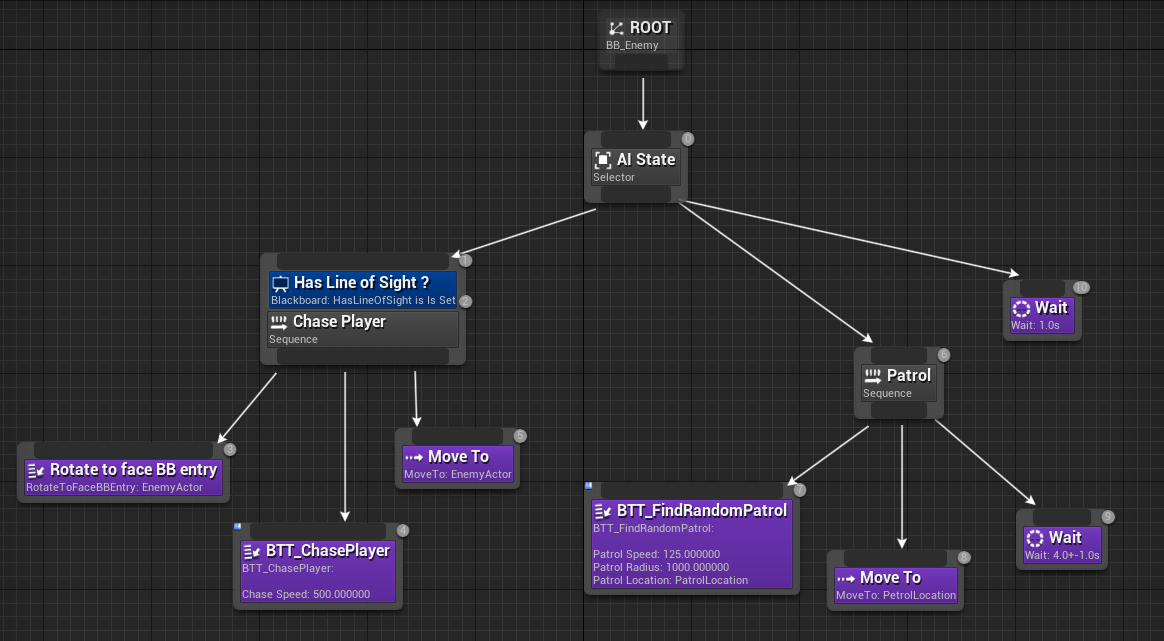
\includegraphics[width=0.75\textwidth]{Imagenes/Bitmap/BTUnreal.png}
    \caption[Ejemplo de \gls{BT} de Unreal Engine]{Ejemplo de un \gls{BT} de Unreal Engine de un \gls{npc} que patruya y persigue al jugador. Fuente: \url{https://dev.epicgames.com/documentation/unreal-engine/behavior-tree-in-unreal-engine---overview} }
    \label{fig:BTUnreal}
\end{figure}

\section{Modelos de lenguaje}
Los modelos de lenguaje son sistemas de \gls{ia} diseñados para comprender, procesar y generar texto.
Al principio se basaban en modelos de lenguaje estadístico, como podemos ver en \cite{Markov} donde los autores cuentan como gracias al análisis de corpus de textos y el uso de n-gramas (una instancia específica de un modelo de Markov) se conseguían estimar las probabilidades de una palabra gracias a un contexto limitado.
Aunque posteriormente surgieron trabajos como \cite{Entropia}, donde usaban el concepto de máxima entropía para que los modelos sean ligeramente sensibles al contexto que mejoraban estos modelos probabilístios, seguían estando muy limitados por su baja capacidad de contexto y nulo razonamiento detrás de las respuestas.

En el trabajo de \cite{PmodelML} se introduce un modelo de lenguaje probabilístico neuronal con el fin de aprender una representación distribuída para cada palabra del vocabulario asociándola con un vector contínuo de características reales y una función de probabilidad condicional de la siguiente palabra dependiendo de su contexto, consiguiendo una reducción de la perplejidad (métrica de los modelos de lenguaje que mide la precisión de predicción de la siguiente palabra) de entre el 10\% y el 20\% y permitiendo aprovechar contextos de entrada más largos y más distribuídos, no solo teniendo en cuenta las N palabras anteriores.
Este trabajo permitió una evolución de modelos de lenguaje probabilísticos a los basados en redes neuronales, como las \gls{RNN} (donde se habla del primero entrenable en \cite{RNNDef}) o las \gls{LSTM} (introducidas en \cite{LSTM}).
En \cite{RNN} se introduce el concepto de las RNN Encoder-Decoder para su uso en traducción de textos, mejorando el flujo de memoria de un \gls{RNN} convencional y consiguiendo un rendimiento significativamente superior gracias a la preservación automática de estructuras semánticas y sintácticas.
A pesar de la mejora que aplicaron las redes neuronales previamente mencionadas frente a los modelos puramente estadísticos, todavía tenían imperfecciones debido al desvanecimiento de contextos en textos amplios o al amplio coste de procesamiento debido a su secuencialidad.
Aún con estas limitaciones los \glspl{LSTM} fueron fundamentales en otro hito de los modelos de lenguaje en el trabajo \cite{ELMo}, en donde los autores introducen la arquitectura ELMo (Embeddings for Language Models), la cual gracias a la suma ponderada de los resultados de las capas \glspl{LSTM} bidireccionales es capaz de generar una representación vectorial de las palabras (\glspl{Embedding}) contextualizada a nivel semántico y sintáctico, a diferencia de las estructuras estáticas que se utilizaban previamente como Word2Vec, introducido en \cite{Word2Vec}.

En el trabajo \cite{Atencion} presentan el modelo Transformer que logra suplir los problemas mencionados de las redes recurrentes.
Esto lo consiguen mediante una arquitectura Encoder-Decoder que contiene unos mecanismos de atención multipropósito y una codificación posicional que inyecta información sobre el órden secuencial, prescindiendo así de los mecanismos de recurrencia.
Los mecanismos de atención logran relacionar cualquier pareja de tokens de una misma secuencia sin importar la distancia física que les separe, permitiendo aprender dependencias a largo alcance y la paralelización del entrenamiento.

\begin{figure}[H]
    \centering
    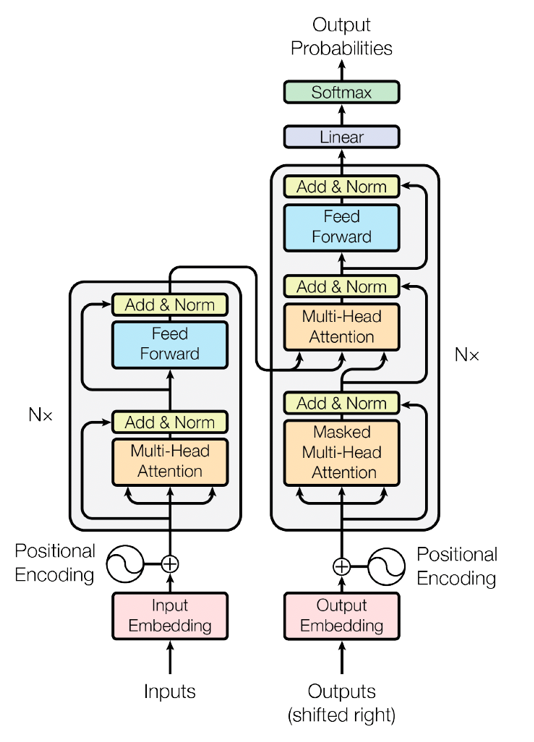
\includegraphics[width=0.75\textwidth]{Imagenes/Bitmap/Transformer.png}
    \caption[arquitectura de un modelo Transformer]{Diagrama de las distintas capas de la arquitectura Transformer. Fuente: \url{https://aws.amazon.com/es/what-is/transformers-in-artificial-intelligence/} }
    \label{fig:BTUnreal}
\end{figure}

Gracias al surgimiento de los Transformers empezaron a aparecer otras arquitecturas que mejoraban las taras del procesamiento del lenguaje natural (NLP por las siglas en inglés de Natural Processing Language).
Podemos destacar la arquitectura BERT, introducida en el trabajo \cite{BERT}.
Esta arquitectura utiliza un codificador Transformer bidireccional multipropósito que para el entrenamiento enmascara de forma aleatoria una serie de tokens (Masked Language Model o MLM) para la predicción del siguiente token según su contexto anterior y posterior, logrando así una bidireccionalidad profunda y logrando un mayor desempeño en tareas como reconocimiento de entidades.
Para ajustar el modelo a una tarea específica se realiza un \gls{Fine-tuning} en el que se cargan los parámetros preentrenados y se vuelven a entrenar todos de forma conjunta (end-to-end) con datos etiquetados de la tarea que se busca.
Esto difiere y mejora otros modelos de representación del lenguaje como ELMo, cuya estrategia de transferencia se basa en la extracción de características (Feature-Based), donde las representaciones contextuales preentrenadas se integran de forma estática como características adicionales dentro de arquitecturas secundarias.

La idea del entrenamiento previo y posterior \gls{Fine-tuning} ya fue mencionada en el artículo \cite{GPT-1}, en donde además introducen el modelo GPT-1.
Este modelo utiliza la arquitectura decodificadora de un Transformer multicapa, el cual en el entrenamiento aplica operaciones de autoatención enmascarada sobre los tokens de contexto para predecir la salida para posteriormente aplicarle \gls{Fine-tuning} para tareas específicas, consiguiendo una mejora respecto a modelos anteriores en tareas como razonamiento del sentido común o comprensión lectora.

Como evolución del modelo anterior podemos ver en el artículo \cite{GPT-3}, donde introducen el modelo GPT-3, cuya arquitectura está basada también un Transformer decoder de 175B de parámetros con la novedad de la introducción de patrones de atención localmente y densamente agrupada de forma alternada.
Este artículo también nos presenta el aprendizaje en contexto (In-Context Learning), el cual se basa en conseguir que un modelo de lenguaje consiga realizar una tarea sin necesidad de cambiar los pesos del modelo mediante \gls{Fine-tuning}, consiguiendo superar la necesidad de grandes cantidades de datos etiquetados.
Esto se puede realizar mediante la descripción de la tarea en lenguaje natural y unos pocos ejemplos (few-shot), un ejemplo (one-shot) o ningún ejemplo (zero-shot).
Con solo este tipo de aprendizaje el modelo fue capaz de mejorar el rendimiento de varias tareas de NLP como traducción o completado de texto así como de conseguir capcaidades emergentes como la aritmética o la generación de noticias sintéticas.

En el artículo \cite{InstructionTuning} presentan el concepto de Instruction Tuning, el cual mejoran las capacidades de aprendizaje en entornos zero-shot.
Lo consiguen mediante el uso de \gls{Fine-tuning} sobre una colección de tareas descritas mediante instrucciones en lenguaje natural, presentando el modelo FLAN basado en un Transformer decoder de 137B parámetros.
De esta forma mejoraron superar en gran medida al modelo GPT-3 en entornos zero-shot y en menor medida en entornos few-shot.

Junto a estas arquitecturas empezaron a surgir aplicaciones que ofrecían el uso de \glspl{LLM} en formato chatbot, como OpenAI\footnote{Página oficial de OpenAI: \url{https://openai.com/es-ES/}} con ChatGPT o Anthropic\footnote{Página oficial de Anthropic: \url{https://www.anthropic.com/}} con Claude así como acceso a sus \glspl{api}, permitiendo a usuarios no expertos el uso de \glspl{LLM} para fines generalistas.
También surgieron frameworks de orquestación de modelos como Langchain\footnote{Página oficial de Langchain: \url{https://www.langchain.com/}} o herramientas que permiten la ejecución de modelos en una máquina local, como es el caso de Ollama \footnote{Página oficial de Ollama: \url{https://ollama.com/}}

Gracias al surgimiento del In-Context Learning y del Instruction Tuning se empezaron a poder pedir tareas específicas a los \glspl{LLM} mediante los prompts, aunque se dan casos donde los modelos no consigan una buena precisión.
Debido a esto se investigaron diferentes métodos de alinear el razonamiento de los modelos a través de refinar el prompt, dando lugar a un conjunto de técnicas que se conocen como \textit{prompt engineering}.
Algunas de estas técnicas ya han sido mencionadas anteriormente, como el zero-shot para casos de Instruction Tuning o few-shot/one-shot para In-Context Learning.
En el artículo \cite{CoT} nos presenta la técnica de Chain-of-Thought, la cual consiste en obligar al modelo a realizar pasos intermedios de razonamiento internamente para mejorar el rendimiento de las tareas complejas.
Otra técnica útil para tareas complejas es Least-To-Most Prompting, presentada en el artículo \cite{LtM} y que consiste en descomponer la tarea general en subtareas sucesivos para ir resolviéndolos de manera incremental.
En la revisión sistemática \cite{RevisionPE} se pueden encontrar 58 técnicas de \textit{prompt engineering}.

Una vez estudiadas las capacidades de razonamiento de los \glspl{LLM} se abrió un camino para el estudio de agentes \glspl{LLM}, sistemas autónomos con modelos de lenguaje integrados que son capaces de percibir, planificar e interactuar con su entorno para completar tareas complejas.
Los autores del artículo \cite{ReAct} presentan el paradigma ReAct, en el que un \gls{LLM} genera alternadamente trazas de razonamiento en lenguaje natural que ayuda al razonamiento para actuar y acciones específicas para la tarea, permitiendo interactuar con el entorno y actuar para razonar.
Otro avance hacia los agentes \gls{LLM} nos lo encontramos en \cite{Toolformer}, donde se puede ver como un agente es capaz de interactuar con \glspl{api} de forma correcta que le permiten realizar mejor tareas como operaciones aritméticas, además de demostrar que se le puede dar una cierta autonomía de interacción con el entorno sin intervención humana a los \glspl{LLM}.
La revisión sistemática de \cite{ToolCallingRev} habla sobre el uso de herramientas (tool calling) en trabajos recientes, organizandolo en cuatro etapas: planificación de la tarea, selección de la herramienta, llamada a la herramienta y respuesta final.
En cuanto a la interacción y planificación de los agentes, el artículo \cite{InnerMonologue} estudia como un \gls{LLM} puede utilizar feedback del entorno para actualizar de forma interna sus planes; mientras que en \cite{LLM+P} argumentan que un \gls{LLM} tiene dificultades en temas de planificación a largo plazo, por lo que proponen usar un planificador clásico entre medias cuando el problema está correctamente formalizado para suplir esta carencia.
Finalmente, en el artículo \cite{AgentesLLM} introduce un sistema multiagente basado en agentes \gls{LLM} sociales con una memoria y la capacidad de recuperar experiencias y de planificar, demostrando que el uso de este tipo de agentes consiguen unas interacciones sociales más creíbles que el uso de agentes clásicos.
En el artículo \cite{AgentesRev} los autores hacen una revisión sistemática sobre agentes autónomos \gls{LLM}.

Para que los agentes \gls{LLM} puedan interactuar con herramientas y recursos externos, en el artículo \cite{MCP} nos habla sobre el protocolo MCP (Model Context Procotol).
Éste es un estándar abierto cuyo objetivo es estandarizar la comunicación bidireccional ente los modelos \gls{LLM} y las fuentes y herramientas externas mediante el desacople de la implementación de las herramientas de su uso.
Para ello se hace el uso de la siguiente arquitectura:
\begin{itemize}
    \item \texttt{MCP Host}: La aplicación que proporciona el entorno de ejecución.
    \item \texttt{MCP Client}: Componente dentro del Host que mantiene la relación con el servidor procesando solicitudes y resupuestas.
    \item \texttt{MCP Server}: Proveedor que expone las herramientas, los recursos y una serie de prompts para plantillas de tareas y flujos de trabajo preconfigurados.
\end{itemize}

En la figura \ref{fig:MCP} podemos ver un diagrama de la arquitectura MCP.

\begin{figure}[H]
    \centering
    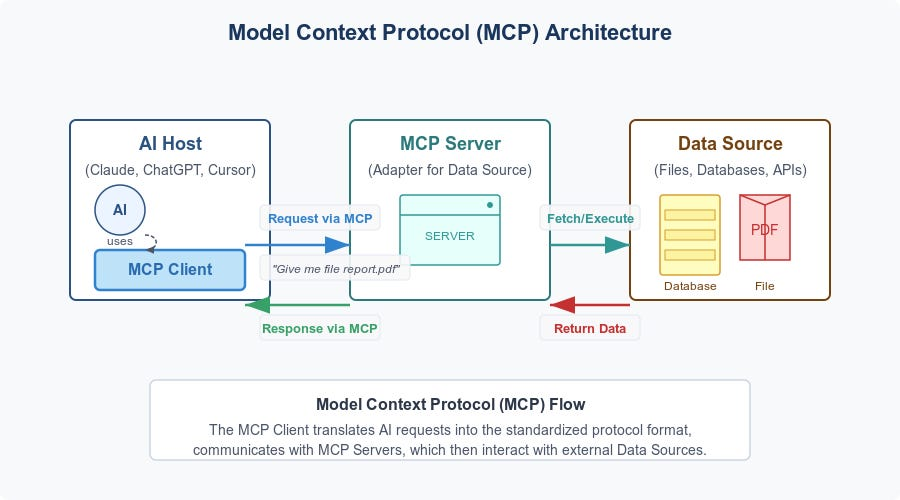
\includegraphics[width=0.75\textwidth]{Imagenes/Bitmap/MCP.jpg}
    \caption[Arquitectura MCP]{Diagrama de la arquitectura MCP. Fuente: \url{https://newsletter.diamant-ai.com/p/model-context-protocol-mcp-explained} }
    \label{fig:MCP}
\end{figure}



\section{Generación automática de comportamientos}
\label{sec:GenCom}

El problema de la generación de comportamientos de forma automática ya existía antes del surgimiento de los \glspl{LLM}, en donde buscaban soluciones mediante algoritmos de \gls{ia} clásica, como podemos ver en \cite{CBR}, donde los autores proponen recuperar y reutilizar comportamientos mediante CBR (siglas de Case-Based Reasoning), construyendo dinámicamente el comportamiento del \gls{npc} a través de una HFSM.
Esta sección se va a centrar en los casos de generaciones automáticas de \glspl{BT}.

\subsection{Generación de \glspl{BT} previos a \glspl{LLM}}
Desde el surgimiento de los \glspl{BT} se ha buscado una forma de automatizar el proceso de su creación.

En el trabajo \cite{IsmaBT} los autores utilizan diferentes técnicas de Machine Learning para generar de forma automática \glspl{BT}.
Primero se utiliza el aprendizaje por demostración (LfD por las siglas en inglés de Learning from Demonstration) de forma que el diseñador realiza la tarea de la que se busca generar el \gls{BT}, registrando las trazas del estado del entorno y las tareas que el \gls{npc} va ejecutando.
Una vez se terminan de recoger esas trazas se generan diferentes modelos de Machine Learning que imitan el comportamiento del agente.
Si este modelo es un árbol de decisión (creado el algoritmo de aprendizaje supervisado C4.5), éste se aplana mediante una búsqueda en profundidad (DFS) para generar reglas lógicas y se unen mediante operadores AND y OR y, usando un algoritmo voraz, simplifica los nodos redundantes hasta construir el \gls{BT} componiéndolo en un nodo de tipo ``Parallel'' o ``Selector''.

En el campo de la programación genética también se han hecho avances en este aspecto.
En el trabajo de \cite{DEFCON} usaron un videojuego comercial donde crean a mano un \gls{BT} inicial cuyas operativas específicas se toman de forma aleatoria.
Es entonces cuando se aplican los algoritmos genéticos sobre esta base del árbol, donde el \textit{crossover} se realiza mediante el intercambio de subramas enteras con el mismo objetivo para dar origen a nuevos comportamientos y la mutación se realiza en parámetros de nodos específicos o insertando nuevas ramas de comportamientos generadas al azar.
La función de \textit{fitness} se entrenó mediante métricas específicas del videojuego, como el potencial defensivo y atacante del \gls{npc}.
Este sistema logró mejorar a la \gls{ia} del videojuego en un 55\% de las partidas, demostrando que los \glspl{BT} generados resultaron ser correctos.
Otros ejemplos del uso de la programación genética para la generación de \glspl{BT} en el ámbito de la robótica la podemos encontrar en trabajos como \cite{BTGen1} o en \cite{BTGen2}, donde además los autores mezclan la programación genética con aprendizaje por demostración.

Finalmente nos encontramos con algoritmos de planificación para la generación de \glspl{BT}, como podemos ver en el trabajo de \cite{BTPlan}.
En este trabajo introducen una metodología para crear y modificar \glspl{BT} en tiempo de ejecución mediante el algoritmo de planificación de retroencadenamiento (Backchaining) en el que se toman un conjunto de acciones con sus precondiciones y postcondiciones y las convierte en \glspl{BT} atómicos bajo un nodo ``Selector''.
Una vez se procesan todas las acciones, se parte de un \gls{BT} que contiene las condiciones finales deseadas y, cada vez que el árbol devuelva un estado ``Failure'' porque el objetivo no se cumple, se reemplaza esa condición por uno de los \glspl{BT} atómicos que sea capaz de resolverla, repitiendo iterativamente este proceso hasta que se de un \gls{BT} correcto.
Si hay una violación de una precondición de otras partes ya predefinidas del árbol, el algoritmo detecta estas colisiones lógicas y las resuelve reordenando el \gls{BT} desplazando el subárbol conflictivo para incrementar su prioridad.

\section{Generación de \glspl{BT} mediante \glspl{LLM} en la robótica}
Dado el gran avance en el campo de los \glspl{LLM} se pueden encontrar varios trabajos que se sirven de éstos para la creación automática de \glspl{BT}, especialmente en el campo de la robótica.

Uno de los primeros trabajos en este ámbito es \cite{llmbrain}, en el que los autores utilizan un modelo basado en Stanford Alpaca 7B al que realizan \gls{Fine-tuning} mediante LoRA (mmodifican únicamente un grupo reducido de pesos de atención) con demostraciones generadas a través de otros modelos más grandes (text-davinci-003), consiguiendo generar \glspl{BT} parecidos a los que pdoría crear un humano para comportamientos robóticos.
Otros trabajos como \cite{BTRob2} siguen una metodología similar en la que utilizan modelos ligeros (de 7B de parámetros) en los que realizan \gls{Fine-tuning} con datasets sintéticos.
En el artículo \cite{LLMBTPlanner} estudia diferentes técnicas de In-Context Learning para generar \glspl{BT} y, además, los compara con modelos de menor tamaño a los que se les ha aplicado \gls{Fine-tuning} y los evalúa en simulaciones, consiguiendo una mayor tasa de aciertos el uso del In-Context Learning.

En el trabajo de \cite{BTRob1} los autores proponen el desarrollo y entrenamiento de un \gls{LLM} especializado únicamente en la generación de \glspl{BT}.
Para ello proponen un pipeline que consta de los siguientes pasos:

\begin{enumerate}
    \item Creación de un dataset mediante la generación de datos sintéticos usando búsquedas en árbol de Monte Carlo (MCTS) combinadas con un sistema \gls{RAG}.
    \item Entrenamiento del modelo mediante aprendizaje auto-supervisado (MLM).
    \item \gls{Fine-tuning} supervisado con datos de instrucciones de usuarios con su respectivo \gls{BT}
    \item Creación de un framework (BTGen Agent) para la generación de los árboles que consta de un módulo de memoria (almacena contextos a corto y largo plazo), módulo de acción (ontología de acciones disponibles), módulo de planificación y módulo de perfil (configura al \gls{LLM} para que adapte roles específicos).
    \item Creación de una metodología de verificación y validación (V\&V) de las capacidades y el rendimiento del \gls{LLM}.
\end{enumerate}

Finalmente los autores del estudio \cite{BTRob3} incorporan a su sistema de generación de \glspl{BT} mediante ChatGPT un ``intérprete de fallos'', el cual permite adaptar en tiempo de ejecución los árboles, consiguiendo una tasa de éxito del 89.6\%.

\section{Generación de \glspl{BT} mediante \glspl{LLM} en videojuegos}

A diferencia del campo de la robótica, la literatura sobre generación de \glspl{BT} para videojuegos es escasa.

En el trabajo de \cite{BTJuegos1} los autores presentan un framework en el que,al igual que en trabajos previos del campo de la robótica, se pueden generar \glspl{BT} a través del lenguaje natural.
Para ello realizan un \gls{Fine-tuning} al modelo ``llama3.1:8B Instruct'' mediante LoRA gracias a un corpus mixto de árboles generados manualmente sobre dos videojuegos comerciales y árboles generados mediante el modelo ``GPT-4o''.
Para generar los árboles se introducen las acciones disponibles en un almacén de vectores \gls{FAISS} y se recuperan mediante etiquetado de roles semántico (SRL).
Mediante pruebas con usuarios se vio que este agente generador alcanzó un 78\% de ejecución correcta en estructuras sencillas, y un 81\% de éxito en estructuras complejas gracias al post-procesamiento.

Para terminar, los autores de \cite{BTJuegos2} proponen un trabajo parecido mediante el modelo ``GPT-5.2'' siguiendo diferentes niveles de detallismo en el prompt del diseñador, donde va desde la descripción explícita de la estructura del \gls{BT} buscado (en donde se consiguió un 100\% de precisión) hasta la delegación completa del diseño, pidiendo una descripción muy vaga del comportamiento buscado.

Esta escasez de trabajos en el ámbito de los videojuegos frente al campo de la robótica hace ver que es conveniente la investigación de esta línea.